%%%%%%%%%%%%%%%%%%%%%%%%%%%%%%%%%%%%%%%%%%%%%%%%%%%%
% LECTURE 26: RADIATION HEAT TRANSFER - ANALYSIS AND APPLICATIONS
%%%%%%%%%%%%%%%%%%%%%%%%%%%%%%%%%%%%%%%%%%%%%%%%%%%%
% \section*{Radiation Heat Transfer - Analysis and Applications}
% \addcontentsline{toc}{section}{Radiation Heat Transfer - Analysis and Applications}

% %%%%%%%%%%%%%%%%%%%%%%%%%%%%%%%%%%%%%%%%%%%%%%%%%%%%
% \subsection*{Course Overview and Final Exam Information}
% \addcontentsline{toc}{subsection}{Course Overview and Final Exam Information}
% %%%%%%%%%%%%%%%%%%%%%%%%%%%%%%%%%%%%%%%%%%%%%%%%%%%%

% The instructor provided several updates about the course structure and final exam:

% \begin{itemize}
%     \item The course is moving quickly through radiation material to ensure coverage of both undergraduate and graduate-level content.
%     \item The last one or two lectures (after this week) will cover advanced graduate-level material that will \textbf{not} be included on the final exam.
%     \item \textbf{Final exam format:}
%     \begin{itemize}
%         \item 5-6 problems to be completed in 2 hours
%         \item Open book exam
%         \item Problems will be comprehensive and similar to previous exams
%         \item Some problems may be challenging (similar to homework difficulty)
%         \item Content will be strictly limited to homework, lecture notes, and previous exams
%         \item Problems may integrate multiple concepts and require multi-step solutions
%         \item Calculations will be manageable with a calculator (no MATLAB required)
%         \item The exam will test conceptual understanding more than computational ability
%         \item The exam may not be curved, but assessment will be based on reasonable expectations and historical performance
%     \end{itemize}
% \end{itemize}

% %%%%%%%%%%%%%%%%%%%%%%%%%%%%%%%%%%%%%%%%%%%%%%%%%%%%
% \subsection*{Review of Radiation Exchange Between Surfaces}
% \addcontentsline{toc}{subsection}{Review of Radiation Exchange Between Surfaces}
% %%%%%%%%%%%%%%%%%%%%%%%%%%%%%%%%%%%%%%%%%%%%%%%%%%%%

% In the previous lecture, we began our discussion of radiation exchange between surfaces within enclosures. Key points to remember:

% \begin{itemize}
%     \item We always work with enclosures where radiation from any surface must terminate within the enclosure (no leakage)
%     \item View factors ($F_{i-j}$) represent the fraction of radiation leaving one surface that directly strikes another surface
%     \item We work with radiosity ($J$) and irradiation ($G$) rather than directly tracking emission/absorption/reflection to avoid tracing complex photon histories
%     \item For practical calculations, we assume surfaces are diffuse, gray, opaque, and have uniform temperature
% \end{itemize}

%%%%%%%%%%%%%%%%%%%%%%%%%%%%%%%%%%%%%%%%%%%%%%%%%%%%
\subsection*{Net Radiation Exchange Between Two Surfaces }
\addcontentsline{toc}{subsection}{Net Radiation Exchange Between Two Surfaces }
%%%%%%%%%%%%%%%%%%%%%%%%%%%%%%%%%%%%%%%%%%%%%%%%%%%%
\begin{wrapfigure}{r}{0.35\textwidth}  % “r” = right side, width = 35% of textwidth
  \vspace{-10pt}                       % tweak vertical position if needed
  \centering
  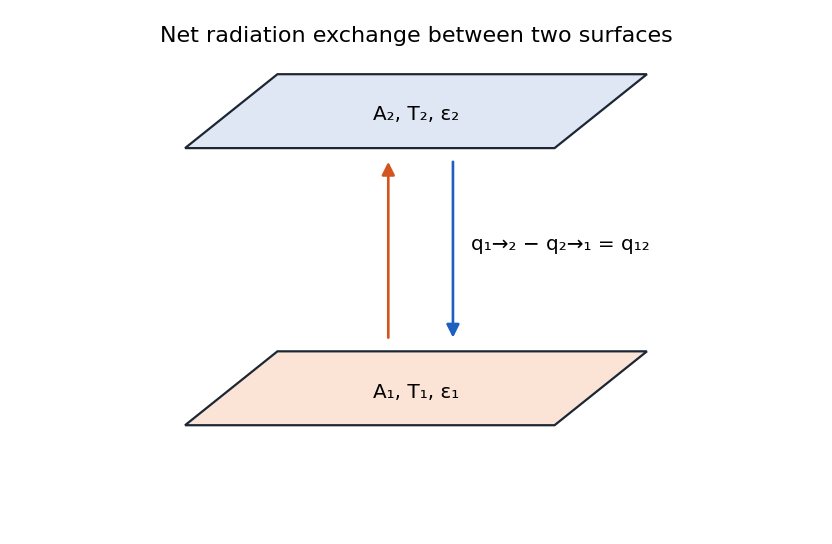
\includegraphics[width=0.25\textwidth]{pics/ratitation_btw_two_surfaces.png}
  \caption{Radiation between surface 1 and 2}
  \label{fig:wrapped}
  \vspace{-10pt}
\end{wrapfigure}
%
The net exchange of radiation between two surfaces is:

\[
    \begin{aligned}
        q_{12} &= q_{1\to 2} - q_{2 \to 1}
        \\[1em ]
        q_{12} & =A_1 F_{12} J_1-A_2 F_{21} J_2
    \end{aligned}
\]

Using reciprocity $\left(A_1 F_{12}=A_2 F_{21}\right)$ :

\[
        q_{12} = \frac{(J_1-J_2)}{1/A_1 F_{12}}
\]

%%%%%%%%%%%%%%%%%%%%%%%%%%%%%%%%%%%%%%%%%%%%%%%%%%%%
\subsubsection*{Sign Convention}
\addcontentsline{toc}{subsubsection}{Sign Convention}
%%%%%%%%%%%%%%%%%%%%%%%%%%%%%%%%%%%%%%%%%%%%%%%%%%%%
It's critical to maintain consistent sign conventions when working with radiation networks:
\begin{itemize}
    \item $q_i$ is positive when heat leaves surface $i$ (cooling)
    \item $q_{i \rightarrow j}$ represents the directional radiation from surface $i$ to surface $j$
    \item $q_{ij}$ represents the net radiation exchange between surfaces $i$ and $j$, with $q_{ij} = -q_{ji}$
\end{itemize}
%
\begin{definition}[Space Resistance]
\paragraph{Formula}
            \[
                    q_{12} = \frac{(J_1-J_2)}{1/A_1 F_{12}}
            \]
\paragraph{Circuit form}
\textbf{
}
\begin{figure}[H]
    \centering
    \begin{circuitikz}
    		% %Grid
    		% \draw[thin, dotted] (0,0) grid (8,8);
    		% \foreach \i in {1,...,8}
    		% {
    		% 	\node at (\i,-2ex) {\i};	
    		% }
    		% \foreach \i in {1,...,8}
    		% {
    		% 	\node at (-2ex,\i) {\i};	
    		% }
    		% \node at (-2ex,-2ex) {0};
    			
    		%Coordinates
    		\coordinate (A) at (3,4);
    		\coordinate (B) at (7,4);
    
    		
    		%Circuit
    		\draw (A) to[resistor, 
                        l^=$1/(A_{1}F_{12})$, 
                        a_= {}, 
                        v_>, 
                        name=r1, 
                        *-*] (B);
    		
    		%Nodes
    		\node[above] at (A) {$J_1$};
    		\node[above] at (B) {$J_2$};
    		
    		% q''
    		\fixedvlen[0.5cm]{r1}{$q_{12}$}		
    
    \end{circuitikz}
\end{figure}
\end{definition}
Space Resistance: Only involves geometry measure of how easily two surfaces exchange thermal radiation.
%%%%%%%%%%%%%%%%%%%%%%%%%%%%%%%%%%%%%%%%%%%%%%%%%%%%
\subsubsection*{Network Construction - Two Surfaces}
\addcontentsline{toc}{subsubsection}{Network Construction - Two Surfaces}
%%%%%%%%%%%%%%%%%%%%%%%%%%%%%%%%%%%%%%%%%%%%%%%%%%%%
For a two-surface enclosure:

\begin{figure}[H]
    \centering
    \ctikzset{bipoles/thickness=2, label distance=5mm, voltage shift = 1}
    \begin{circuitikz}
    		% %Grid
    		% \draw[thin, dotted] (0,0) grid (8,8);
    		% \foreach \i in {1,...,8}
    		% {
    		% 	\node at (\i,-2ex) {\i};	
    		% }
    		% \foreach \i in {1,...,8}
    		% {
    		% 	\node at (-2ex,\i) {\i};	
    		% }
    		% \node at (-2ex,-2ex) {0};
    			
    		%Coordinates
    		\coordinate (A) at (3,4);
    		\coordinate (B) at (6,4);
            \coordinate (C) at (9,4);
            \coordinate (D) at (12,4);
    		
    		%Circuit
    		\draw (A) to[resistor, 
                        l^=$\frac{1-\varepsilon_1}{\varepsilon_1 A_1}$, 
                        a_= {}, 
                        v_>, 
                        name=r1, 
                        o-*] (B);
    		\draw (B) to[resistor, 
                        l^=$\frac{J_1-J_2}{1/A_1F_{12}}$, 
                        a_= {}, 
                        v_>, 
                        name=r2, 
                        *-*] (C);  
    		\draw (C) to[resistor, 
                        l^=$\frac{1-\varepsilon_2}{\varepsilon_2 A_2}$, 
                        a_= {}, 
                        v_>, 
                        name=r3, 
                        *-o] (D); 
    		%Nodes
    		\node[above] at (A) {$E_{b1}$};
    		\node[above] at (B) {$J_1$};
    		\node[above] at (C) {$J_2$};
    		\node[above] at (D) {$E_{b2}$};
            
    		% q''
    		\fixedvlen[0.5cm]{r1}{$q_{1}$}
            \fixedvlen[0.5cm]{r2}{$q_{12}$}
            \fixedvlen[0.5cm]{r3}{$-q_{2}$}
            
    \end{circuitikz}
\end{figure}
%%%%%%%%%%%%%%%%%%%%%%%%%%%%%%%%%%%%%%%%%%%%%%%%%%%%
\subsubsection*{Network Construction - Three Surfaces}
\addcontentsline{toc}{subsubsection}{Network Construction - Three Surfaces}
%%%%%%%%%%%%%%%%%%%%%%%%%%%%%%%%%%%%%%%%%%%%%%%%%%%%
For a three-surface enclosure:

\begin{figure}[H]
    \centering
    \ctikzset{bipoles/thickness=2, label distance=5mm, voltage shift = 1}
    \begin{circuitikz}
    		% %Grid
    		% \draw[thin, dotted] (0,0) grid (8,8);
    		% \foreach \i in {1,...,8}
    		% {
    		% 	\node at (\i,-2ex) {\i};	
    		% }
    		% \foreach \i in {1,...,8}
    		% {
    		% 	\node at (-2ex,\i) {\i};	
    		% }
    		% \node at (-2ex,-2ex) {0};
    			
    		%Coordinates
    		\coordinate (A) at (3,4);
    		\coordinate (B) at (7,4);
            \coordinate (C) at (11,4);
            \coordinate (D) at (15,4);
            \coordinate (E) at (9,1.5);
    		\coordinate (F) at (9,-1.25);
            
    		%Circuit
    		\draw (A) to[R, 
                        l^=$\frac{1-\varepsilon_1}{\varepsilon_1 A_1}$, 
                        a_= {}, 
                        v_>, 
                        name=r1, 
                        o-*] (B);
    		\draw (B) to[R, 
                        l^=$\frac{J_1-J_2}{1/A_1F_{12}}$, 
                        a_= {}, 
                        v_>, 
                        name=r2, 
                        *-*] (C);  
    		\draw (C) to[R, 
                        l^=$\frac{1-\varepsilon_2}{\varepsilon_2 A_2}$, 
                        a_= {}, 
                        v_<, 
                        name=r3, 
                        *-o] (D); 
    		\draw (B) to[R, 
                        l_=$\frac{J_1-J_3}{1/A_1F_{13}}$, 
                        i_> ={$q_{13}$},
                        current/distance=-1.5,
                        a_= {}, 
                        %v^>, 
                        name=r4, 
                        *-*] (E); 
    		\draw (C) to[R, 
                        i^> ={$q_{23}$},
                        current/distance=-1.5,
                        l^=$\frac{J_2-J_3}{1/A_2F_{23}}$, 
                        a_= {}, 
                        %v_>,
                        name=r5, 
                        *-*] (E);
    		\draw (E) to[R, 
                        l^=$\frac{1-\varepsilon_3}{\varepsilon_3 A_3}$, 
                        a_= {}, 
                        v_<, 
                        name=r6, 
                        *-o] (F);
    		%Nodes
    		\node[above] at (A) {$E_{b1}$};
    		\node[above] at (B) {$J_1$};
    		\node[above] at (C) {$J_2$};
    		\node[above] at (D) {$E_{b2}$};
            \node[below left] at (E) {$J_3$};
            \node[right] at (F) {$E_{b3}$};
    		% q''
    		\fixedvlen[0.5cm]{r1}{$q_{1}$}
            \fixedvlen[0.5cm]{r2}{$q_{12}$}
            \fixedvlen[0.5cm]{r3}{$q_{2}$}
            \fixedvlen[0.5cm]{r6}{$q_{3}$}
            
    \end{circuitikz}
\end{figure}
\ctikzset{bipoles/thickness=2, label distance=1mm, voltage shift = 1}

For each additional surface, we add:
\begin{itemize}
    \item A new $E_{bi}$ and $J_i$ node pair
    \item A surface resistance connecting $E_{bi}$ to $J_i$
    \item Space resistances connecting $J_i$ to all other $J$ nodes
\end{itemize}

%%%%%%%%%%%%%%%%%%%%%%%%%%%%%%%%%%%%%%%%%%%%%%%%%%%%
\subsection*{Network Analysis Method}
\addcontentsline{toc}{subsection}{Network Analysis Method}
%%%%%%%%%%%%%%%%%%%%%%%%%%%%%%%%%%%%%%%%%%%%%%%%%%%%

To solve a radiation network:

\begin{enumerate}
    \item Identify the number of unknowns (typically one per surface - either $T_i$ or $q_i$)
    \item Write energy balance equations at each $J$ node using Kirchhoff's current law
    \item For each $J$ node: $q_i = \sum_{j \neq i} q_{ij}$ (what leaves a surface must distribute to all other surfaces)
    \item Express these in terms of potentials and resistances:
    \[
        \frac{E_{b, i}-J_i}{\frac{1-\varepsilon_i}{\varepsilon_i A_i}}= \sum_{j \neq i} \frac{J_i - J_j}{\frac{1}{A_i F_{i j}}}
    \]
    \item Solve the resulting system of equations
\end{enumerate}

For an $N$-surface enclosure, you'll need to solve a system of $N$ equations with $N$ unknowns.

\begin{itemize}
    \item For a known temperature distribution, solve for heat transfer rates
    \item For a known heat transfer distribution, solve for surface temperatures
\end{itemize}
%
\paragraph{Key Points:}
\[
        \left\{\begin{array}{lccl}
            q_{i \to j} = A_{i}J_{i}F_{ij} &  &&\text {Ratio of radiation ($J=E_b + \rho G$ leaves $i$ and falls on $j$} 
            \\[1em]
            q_{ij} = q_{i \to j} - q_{j \to i}&&& \text{Net radiation exchange between $i$ and $j$ (Leaving $i$ is positive)}
            \\[1em]
            q_i=\sum_{j=1}^N q_{i j} &&& \text {Total net radiation loss for $i$}
        \end{array}
        \right.
\]
Therefore,
\[
\boxed{
    \begin{aligned}
        &q_{ij} = - q_{ji}
        \\[1em]
        &q_{i \to j} \neq q_{j \to i} \qquad(\textit{unless $J_i = J_j$})
        \\[1em]
        &\sum_{i=1}^N q_i = \sum_{i=1}^N\sum_{j=1}^N q_{ij}= 0 \qquad \text{good for checking after solving}
    \end{aligned}
    }
\]

%%%%%%%%%%%%%%%%%%%%%%%%%%%%%%%%%%%%%%%%%%%%%%%%%%%%
\subsection*{Re-radiating Surfaces}
\addcontentsline{toc}{subsection}{Re-radiating Surfaces}
%%%%%%%%%%%%%%%%%%%%%%%%%%%%%%%%%%%%%%%%%%%%%%%%%%%%

A reradiating surface is one that:
\begin{itemize}
    \item Is thermally insulated from conduction and convection
    \item Has no internal heat generation
    \item Participates only in radiation heat transfer
    \item Must achieve a temperature where the net radiation exchange equals zero
\end{itemize}

For a reradiating surface $i$, we have:
\begin{itemize}
    \item $q_i = 0$ (no net heat transfer to/from the surface)
    \item $E_{bi} = J_i$ (the radiosity equals the blackbody emission)
\end{itemize}

This significantly simplifies the network, as we can eliminate the $E_{bi}$ node and directly work with the $J_i$ node. The surface resistance becomes irrelevant since there is no potential difference across it.
%
\begin{figure}[H]
    \centering
    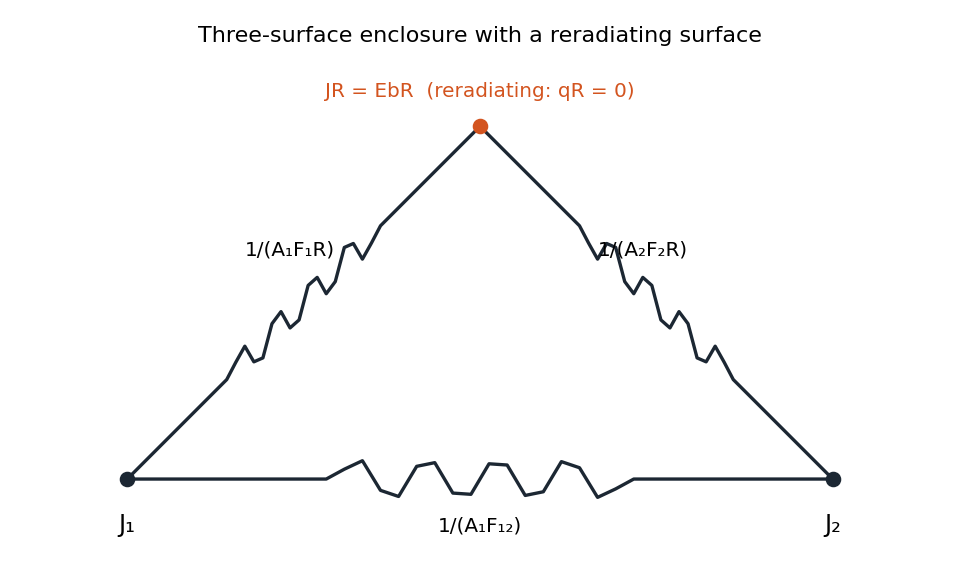
\includegraphics[width=0.5\linewidth]{pics/re_radiation_surface.png}
    \caption{Schematic of a three-surface enclosure with one surface reradiating}
\end{figure}
%
\begin{figure}[H]
    \centering
    \ctikzset{bipoles/thickness=2, label distance=5mm, voltage shift = 1}
    \begin{circuitikz}
    		% %Grid
    		% \draw[thin, dotted] (0,0) grid (8,8);
    		% \foreach \i in {1,...,8}
    		% {
    		% 	\node at (\i,-2ex) {\i};	
    		% }
    		% \foreach \i in {1,...,8}
    		% {
    		% 	\node at (-2ex,\i) {\i};	
    		% }
    		% \node at (-2ex,-2ex) {0};
    			
    		%Coordinates
    		\coordinate (A) at (3,4);
    		\coordinate (B) at (7,4);
            \coordinate (C) at (11,4);
            \coordinate (D) at (15,4);
            \coordinate (E) at (9,7);
            
    		%Circuit
    		\draw (A) to[R, 
                        l^=$\frac{1-\varepsilon_1}{\varepsilon_1 A_1}$, 
                        a_= {}, 
                        v_>, 
                        name=r1, 
                        o-*] (B);
    		\draw (B) to[R, 
                        l_=$\frac{1}{A_1F_{12}}$, 
                        a_= {}, 
                        v^>, 
                        name=r2, 
                        *-*] (C);  
    		\draw (C) to[R, 
                        l^=$\frac{1-\varepsilon_2}{\varepsilon_2 A_2}$, 
                        a_= {}, 
                        v_<, 
                        name=r3, 
                        *-o] (D); 
    		\draw (B) to[R, 
                        l^=$\frac{1}{A_1F_{1R}}$, 
                        i^> ={$q_{1R}$},
                        current/distance=-1.5,
                        a_= {}, 
                        %v^>, 
                        name=r4, 
                        *-*] (E); 
    		\draw (C) to[R, 
                        i_> ={$q_{2R}$},
                        current/distance=-1.5,
                        l_=$\frac{1}{A_2F_{2R}}$, 
                        a_= {}, 
                        %v_>,
                        name=r5, 
                        *-o] (E);

    		%Nodes
    		\node[above] at (A) {$E_{b1}$};
    		\node[below] at (B) {$J_1$};
    		\node[below] at (C) {$J_2$};
    		\node[above] at (D) {$E_{b2}$};
            \node[above] at (E) {$E_{bR} = J_R$};
    		% q''
    		\fixedvlen[0.5cm]{r1}{$q_{1}$}
            \fixedvlen[0.5cm]{r2}{$q_{12}$}
            \fixedvlen[0.5cm]{r3}{$q_{2}$}
            
    \end{circuitikz}
\end{figure}
Considering the entire circuit, we can simply find heat transfer as follow:
\[
        q_1 = - q_2 = \frac{E_{b1}-E_{b2}}{R_{s1} + [R_{13}+R_{23}]\parallel R_{12} + R_{s2}}
\]
where
\[
    \begin{aligned}
        R_{s1} &= \frac{1-\varepsilon_1}{\varepsilon_1 A_1}
        \\[1em]
        R_{s2} &= \frac{1-\varepsilon_2}{\varepsilon_2 A_2}
        \\[1em]
        [R_{13}+R_{23}]\parallel  R_{12} &= \frac{1}{A_1 F_{12}+\left[\left(1 / A_1 F_{1 R}\right)+\left(1 / A_2 F_{2 R}\right)\right]^{-1}}
    \end{aligned}
\]
% An important insight: The temperature of a re-radiating surface depends only on the temperatures of other surfaces in the enclosure and the view factors, not on its own emissivity. This is analogous to the concept in circuit theory where a point with zero current (floating potential) adopts the potential of its connected nodes regardless of the resistance values.

%%%%%%%%%%%%%%%%%%%%%%%%%%%%%%%%%%%%%%%%%%%%%%%%%%%%
\subsection*{Important Considerations for Radiation Resistance}
\addcontentsline{toc}{subsection}{Important Considerations for Radiation Resistance}
%%%%%%%%%%%%%%%%%%%%%%%%%%%%%%%%%%%%%%%%%%%%%%%%%%%%

When working with radiation resistances, several important considerations must be kept in mind:

\begin{enumerate}
    \item \textbf{Units:} Radiation resistances have units of $\text{m}^{-2}$, which is different from conduction or convection resistances. This means they cannot be directly combined in a single network without proper conversion.
    
    \item \textbf{Temperature potential:} Radiation networks use $\sigma T^4$ as the potential rather than $T$, making them fundamentally different from conduction/convection networks.
    
    \item \textbf{Dimensional consistency:} When solving networks, ensure all terms maintain proper dimensional consistency.
    
    \item \textbf{Network reduction:} While circuit reduction techniques (series, parallel) can sometimes be applied, it's only valid for specific cases where the heat flow path is effectively one-dimensional.
    
    \item \textbf{Mixing modes:} Never directly connect radiation resistances to conduction/convection resistances in a single network without proper conversion - this would be like "adding apples and oranges."
\end{enumerate}

%%%%%%%%%%%%%%%%%%%%%%%%%%%%%%%%%%%%%%%%%%%%%%%%%%%%
\subsection*{Multi-Mode Heat Transfer}
\addcontentsline{toc}{subsection}{Multi-Mode Heat Transfer}
%%%%%%%%%%%%%%%%%%%%%%%%%%%%%%%%%%%%%%%%%%%%%%%%%%%%

Many practical problems involve multiple heat transfer modes (conduction, convection, and radiation) simultaneously. To handle such problems:

\begin{enumerate}
    \item Draw a control volume that captures all relevant heat transfer mechanisms
    \item Apply energy conservation to this control volume
    \item Use consistent sign conventions across all modes (e.g., positive for heat leaving the surface)
    \item Consider appropriate boundary conditions for each mode
\end{enumerate}
%
\begin{figure}[H]
    \centering
    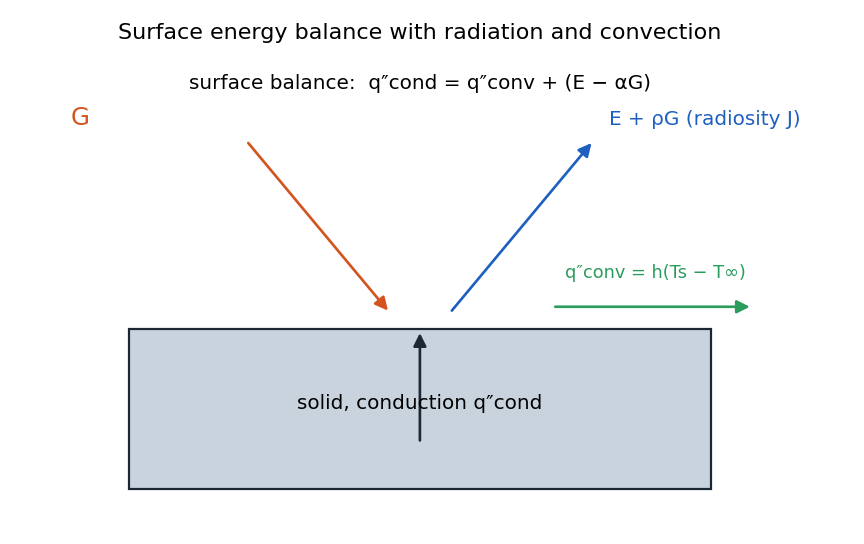
\includegraphics[width=0.3\linewidth]{pics/multimode_heat_transfer.png}
    \caption{Surface energy balance}
\end{figure}
%
For a steady-state surface energy balance with consistent sign convention (positive for heat leaving):
\[
    \begin{aligned}
    & \cancelto{0}{\dot{E}_{\text{in}}}-\dot{E}_{\text {out }}+\dot{E}_{\text {gen }}= \cancelto{0}{\dot{\dot{E}}_{s t}}
    \\[0.5em]
    & \dot{q}_{i, \text { ext}}=q_{i, \text { rad }}+q_{i, \text { conv. }}+q_{i, \text { cond. }}
    \end{aligned}
\]
\textit{Note:} 
\begin{itemize}
    \item for $q_{i, \text { rad }}, q_{i, \text { conv }}$ and $q_{i, \text { cond, }}$, positive mean surface losses energy.
    \item $q_{i \text {, rad }}$ is the $q_i$ in previous radiation network. 
    \item $q_{i, \text { ext }}=q_{i, \text { rad }}+q_{i, \text { conv }}+q_{i, \text { cond }}$
    holds at any time, ie., transient and steady state..
\end{itemize}
%%%%%%%%%%%%%%%%%%%%%%%%%%%%%%%%%%%%%%%%%%%%%%%%%%%%%
\subsubsection*{Solution Strategy for Multi-Mode Problems}
\addcontentsline{toc}{subsubsection}{Solution Strategy for Multi-Mode Problems}
%%%%%%%%%%%%%%%%%%%%%%%%%%%%%%%%%%%%%%%%%%%%%%%%%%%%%

When solving problems with multiple heat transfer modes:

\begin{enumerate}
    \item Solve the radiation network first (radiation responds essentially instantaneously)
    \item Use the resulting heat fluxes as boundary conditions for conduction/convection
    \item Apply energy conservation at each surface
    \item For complex geometries, numerical methods may be required
\end{enumerate}

The instructor emphasized that radiation is effectively a "rigid" constraint that responds at the speed of light, making it appropriate to solve first and then use as a boundary condition for slower processes.

% \subsubsection*{Examples of Concentrated Surface Heating ($Q_{\text{gen}}$)}
% \addcontentsline{toc}{subsubsection}{Examples of Concentrated Surface Heating ($Q_{\text{gen}}$)}

% Various physical processes can be modeled as concentrated surface heat generation:

% \begin{itemize}
%     \item Nuclear decay at a surface
%     \item Photothermal heating (laser or light absorption)
%     \item Solar panel absorption
%     \item Surface chemical reactions
%     \item Evaporation/condensation at interfaces
% \end{itemize}

% The applicability depends on whether the process occurs within a thin layer that can be reasonably approximated as a surface phenomenon.

\paragraph{Example: } Consider a very long enclosure with a uniform square cross section as shown below. One of the view factors is known as $\boldsymbol{F}_{13} \approx 0.4$. Find the rest of the view factors.

\textbf{
}

\textit{solution:} We have
\begin{itemize}
    \item Due to the flat surfaces, all self-view factors are zero: $F_{11} = F_{22} = F_{33} = F_{44} = 0$
    \item Due to symmetry in the square enclosure:
    \begin{itemize}
        \item Opposite surfaces: $F_{13} = F_{31} = F_{24} = F_{42} = 0.4$
        \item Adjacent surfaces: $F_{12} = F_{21} = F_{23} = F_{32} = F_{34} = F_{43} = F_{41} = F_{14} = 0.3$
    \end{itemize}
    \item Verification: For each surface, the sum of view factors equals 1
    \[
    F_{i1} + F_{i2} + F_{i3} + F_{i4} = 0 + 0.3 + 0.4 + 0.3 = 1
    \]
\end{itemize}
%
\begin{table}[H]
    \centering
    \begin{tabular}{|c|c|c|c|c|}
    \hline$F_{i j}$ & $i=1$ & $i=2$ & $i=3$ & $i = 4$ \\
    \hline$j=1$ & 0 & 0.3 & 0.4 & 0.3 \\
    \hline$j=2$ & 0.3 & 0 & 0.3 & 0.4 \\
    \hline$j=3$ & 0.4 & 0.3 & 0 & 0.3 \\
    \hline$j=4$ & 0.3 & 0.4 & 0.3 & 0 \\
    \hline
    \end{tabular}
\end{table}

% %%%%%%%%%%%%%%%%%%%%%%%%%%%%%%%%%%%%%%%%%%%%%%%%%%%%
% \subsection*{Verification of Reradiating Surface Behavior}
% \addcontentsline{toc}{subsection}{Verification of Reradiating Surface Behavior}
% %%%%%%%%%%%%%%%%%%%%%%%%%%%%%%%%%%%%%%%%%%%%%%%%%%%%

% The assumption that a surface is reradiating should be verified after calculating its temperature. Once you know the temperature:

% \begin{enumerate}
%     \item Calculate the expected conduction and convection heat transfer
%     \item Compare to the radiation heat transfer
%     \item If conduction/convection is negligible compared to radiation, the reradiating assumption is valid
%     \item If not, a multi-mode analysis is required
% \end{enumerate}

% There is no "perfect insulation" in reality - the assumption should be validated based on the specific conditions of the problem.

